%----------------------------------------------------------------------------------------------------------------------------------------------------------%
\chapter{Introduction}
%----------------------------------------------------------------------------------------------------------------------------------------------------------%
\section{An overview of the study}

%----------------------------------------------------------------------------------------------------------------------------------------------------------%
\section{Bacteria and bacterial infections}
\paragraph{Bacteria} are prokaryote organisms, generally single-celled, which are part of the Monera animal kingdom. Their sizes range from between \SI{30}{\micro\metre} and \SI{100}{\micro\metre} and are ubiquitous\footnote{Ubiquitous: found everywhere} organisms. This form of life is believed to be the first one to have ever appeared on Earth, as well as the one responsible for the oxigen-rich atmosphere the Earth currently has. Some species are hard to culture in a laboratory environment, but generally, those that can be cultured in a controlled environment are grown in agar plates\cite{MicrobioMed}. \newline
Agar is used as a place to grow bacteria due to the fact that it is indigestible for the majority of bacteria, yet it keeps them humid and, together with growth mediums, such as Lysogeny Broth, bacteria thrive in this environment, allowing them to proliferate and create colonies, which can be seen to the naked eye. Sometimes, together with the growth medium, additives such as mannitol salt are added. These are used to improve or impede bacterial growth, modify their conditions so they develop differently or as an identification tool. For example, \emph{Staphyloccus Aureus} ferments it, producing acid, which in turn decolorates the plate from red to yellow.
\paragraph{Pathogenic bacteria} are bacteria that have the ability to cause disease\footnote{''A disease is a particular abnormal condition that negatively affects the structure or function of all or part of an organism, and that is not immediately due to any external injury.''\cite{dorlands:001}}. These are not the most common type of bacteria, as the majority of them are either harmless or benefitial to the human body through symbiosis, such as the bacteria that help with digestion in the stomach\footnote{citation needed}.

%----------------------------------------------------------------------------------------------------------------------------------------------------------%
\section{The enemy: Staphylococcus aureus}
\paragraph{}\emph{Staphylococcus aureus} (also known as Staph) is a GRAM-positive bacteria, the most virulent and studied of its genus\footnote{citation needed, got to check the proper terminology}. Some of its distinctive characteristics include having a very thick glycopeptide wall, which allows it to withstand extreme temperatures and osmotic pressures, therefore rendering most classic methods of food conservation (such as cooking, smoking, freezing or salting\footnote{citation needed}) completely useless against said bacteria;  a protein A capsid, which binds to many eukaryote organism. It's an extremely resistant (and thus ubiquitous) bacteria. It can be found in human skin and mucotic surfaces (such as the mouth or the nose), as well as in certain foods such as ham (cooked or curated), eggs, raw and cooked dough, as well as in poultry.
\paragraph{}
\begin{wrapfigure}{r}{0.5\textwidth}\begin{center}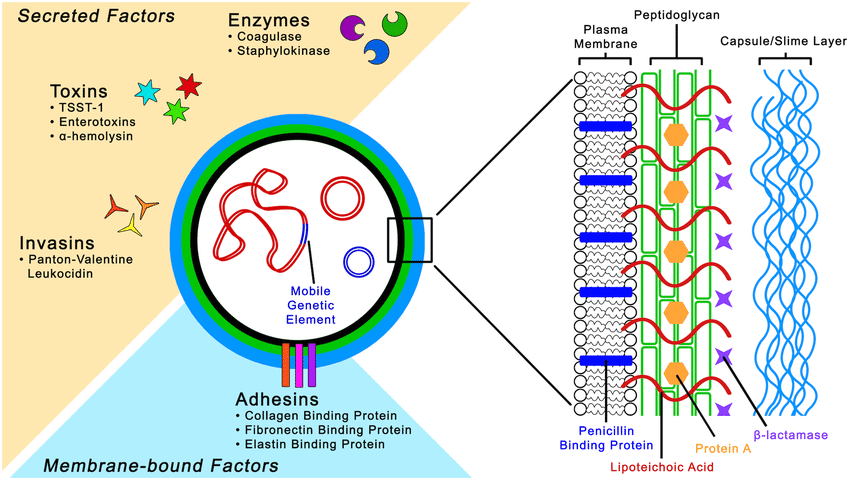
\includegraphics[width=0.48\textwidth]{staph_parts.png}\end{center}\caption{Parts of Staphylococcus aureus. Source: [source]}\end{wrapfigure}
Staphylococcus Aureus has three main parts to its virulence: its cell wall, its membrane-bound factors and its secreted factors. Staph's \textbf{cell wall} is made up of three parts, going from inside to the outside of the cell: a plasma membrane, a peptidoglycan layer and a slime (sometimes also called capsule) layer.\newline %source: https://www.genome.gov/genetics-glossary/Plasma-Membrane%
The plasma membrane consists of a lipid bilayer that is semipermeable\footnote{Semipermeable: it lets water and ions through, but not other molecules. This transport will always be in favour of the pressure gradient, which means that it cannot insert any kind of substance into an environment that has a higher pressure than the other side}, which regulates the transport of materials entering and exiting the cell. Integrated inside them are a type of integral protein called penicillin-binding protein (PBP), amongst other  proteins such as protein channels. We will only talk about PBPs because they are the Achilles's Heel of bacteria, as long as you know how to exploit it. Whilst the name implies PBPs are only sensible to penicillin, the name actually comes because that's how they were discovered, and in fact could be resistant to it but sensible to other antibiotic agents. Variations in this protein may lead in some cases to antibiotic resistance, such as MRSA (\emph{Methicillin-Resistant Staphylococcus Aureus}), a variation of Staph that is the result of a variation in this protein called PBP2A. The different variations of \emph{Staphylococcus Aureus} will be discussed in more detail in a following section. \newline
\emph{Staphylococcus aureus}, like all other members of the \emph{Staphylococcus} family, have very thick peptidoglycan layers. This grants them protection from extreme temperatures and high osmotic pressures, which means these bacteria can colonise cooked food and food that has been salted. The most notable example is ham, either cooked, smoked or cured.
%----------------------------------------------------------------------------------------------------------------------------------------------------------%
\section{The enemy's attacks}
\paragraph{}One of Staph's most notorious abilities is using the body's own proteins to disguise itself and thus avoid detection and phagocytosis by the host's immune system. It accomplishes this task by using an enzyme called coagulase, which enables the transformation of fibrinogen (a glycoproteic complex produced in the liver and present in the blood of all vertebrates) to fibrin (fibrinogen after being stimulated by either thrombin or \emph{staphylothrombin}, the result of a molecular pathway stimulated by coagulase. It helps in clotting the blood in the event of vascular or tissue injury)[source: microbiology medical]. Only 11 other \emph{Staphylococcus} family members are coagulase-positive. To test for this enzyme in the laboratory there are two main methods which are usually combined: culture of the sample on a Baird-Parker agar medium, a selective and differential medium which contains lithium chloride and tellurite as to inhibit the growth of other microbes. It also includes pyruvate and glycine, which promote the growth of \emph{Staphylococci} colonies, showing in colour black and with an opaque zone around the colony. This opaque zone represents the effect of the coagulase. Another way to test for coagulase is to perform a coagulase test. This test generally requires a small quantity (generally 2 mL) of sheep blood serum, which will gelatinise if coagulase is present.
\paragraph{}
%----------------------------------------------------------------------------------------------------------------------------------------------------------%
\section{Our weapons}
\paragraph{}I'll write this back at the UDG library with the book  I used to make that thing. If I can't, I will just find the scanned pages and work my way backwards from there.
%----------------------------------------------------------------------------------------------------------------------------------------------------------%
\section{Risk assessment and prevention}
\paragraph{}Staph is considered a Biosecurity Level (BSL) 2 pathogenic bacteria. This means that the it is associated with a human disease that can pose a moderate health hazard. In a laboratory where BSL-2 pathogens are handled, regular lab rules should be followed (mechanical pipetting only, hand washing, prohibiting the consumption of food and drinks in the lab, proper PPE use...), as well as avoiding splashes or aerosols, biohazard warning signs present on all material used, as well as proper surface and material disinfection via the use of autoclave or alternative decontamination method.[source: book] The risks associated with this bacteria were assessed following the protocol designated by the World Health Organisation [cite], and proper security measures were followed at all times when handling biohazardous material. No incidents occurred during the research part of this project, and the protocol defined previous to the start was followed to a T.
%----------------------------------------------------------------------------------------------------------------------------------------------------------%


